\section{Aufbau und Durchführung} % (fold)
\label{sec:aufbau_und_durchf_hrung}

	Zur Messung der ersten beiden Versuchsteile wurden hauptsächlich ein CCD-Detektor und ein Computer mit dem installierten Programm \textit{MaxIm DL Pro 6} verwendet.
	Der CCD-Detektor wurde durch eine vorhandene Kappe abgedunkelt, um es zu ermöglichen Bias- und Dunkelstrombilder aufnehmen zu können und an den Rechner angeschlossen.
	Das Programm ermöglichte die Steuerung der CCD-Kamera und die Verarbeitung von gesendeten Signalen.
	Das Spektrometer bestand wie in den Grundlagen beschrieben aus der CCD-Kamera mit einem vorangestellten Gitter und drei übereinander liegenden Blenden.
	Über eine eingebaute Mechanik ließ sich der Winkel zwischen Gitter und CCD und somit der betrachtete Wellenlängenbereich einstellen,
	Um die Abhängigkeit der Auflösung von der Gitterkonstanten zu ermitteln, wurden abwechselnd zwei Gitter mit $200$ bzw. $900$ Linien pro $\unit{mm}$ verwendet.

	\subsection{Bestimmung des Ausleserauschens des CCD-Detektors} % (fold)
	\label{sub:bestimmung_des_ausleserauschens_des_ccd_detektors}
	
		Das Ausleserauschen des CCD-Detektors wurde mit Hilfe von Bias-Aufnahmen bestimmt.
		Diese entstanden bei geschlossener Blende und sehr kurzer Belichtungszeit und ergeben Bilder, die nur aus dem Biaslevel und zufälligen Rauschen bestehen.
		Um das Biaslevel aufzunehmen, wurden nacheinander einhundert Bias-Aufnahmen bei konstanter Temperatur erstellt, gemittelt und im BIAS-Mean-Bild gespeichert. 
		Die Intensität des zufälligen Rauschens konnte durch Abzug des Bias-Mean von einer willkürlichen Bias-Aufnahme gemessen werden.

	% subsection bestimmung_des_ausleserauschens_des_ccd_detektors (end)


	\subsection{Dunkelstromaufnahme} % (fold)
	\label{sub:dunkelstromaufnahme}

		Hierzu wurde die Blende der CCD geschlossen gehalten und nacheinander bei steigender Temperatur und konstanter Belichtungszeit von 5 Minuten wurden die verschiedenen Dunkelstrombilder erzeugt. 
		Nach Abzug einer anschließend geschossenen Bias-Aufnahme konnte die Intensität des thermischen Dunkelstromes ermittelt werden.
		Die Einstellung auf die gewünschte Temperatur erfolgte mit Hilfe eines Peltier-Elements.
		Diese erreichen für gewöhnlich Temperaturen von bis zu 30 Grad Celsius unter Umgebungstemperatur.
		Die CCD-Kamera wurde mit einer zusätzlichen Abdeckung versehen um neben der geschlossenen Blende das Umgebungslicht abzuschirmen.
		Der Aufbau ist in Bild \ref{ccd_solo} zu sehen.


		\begin{figure}
			\center
			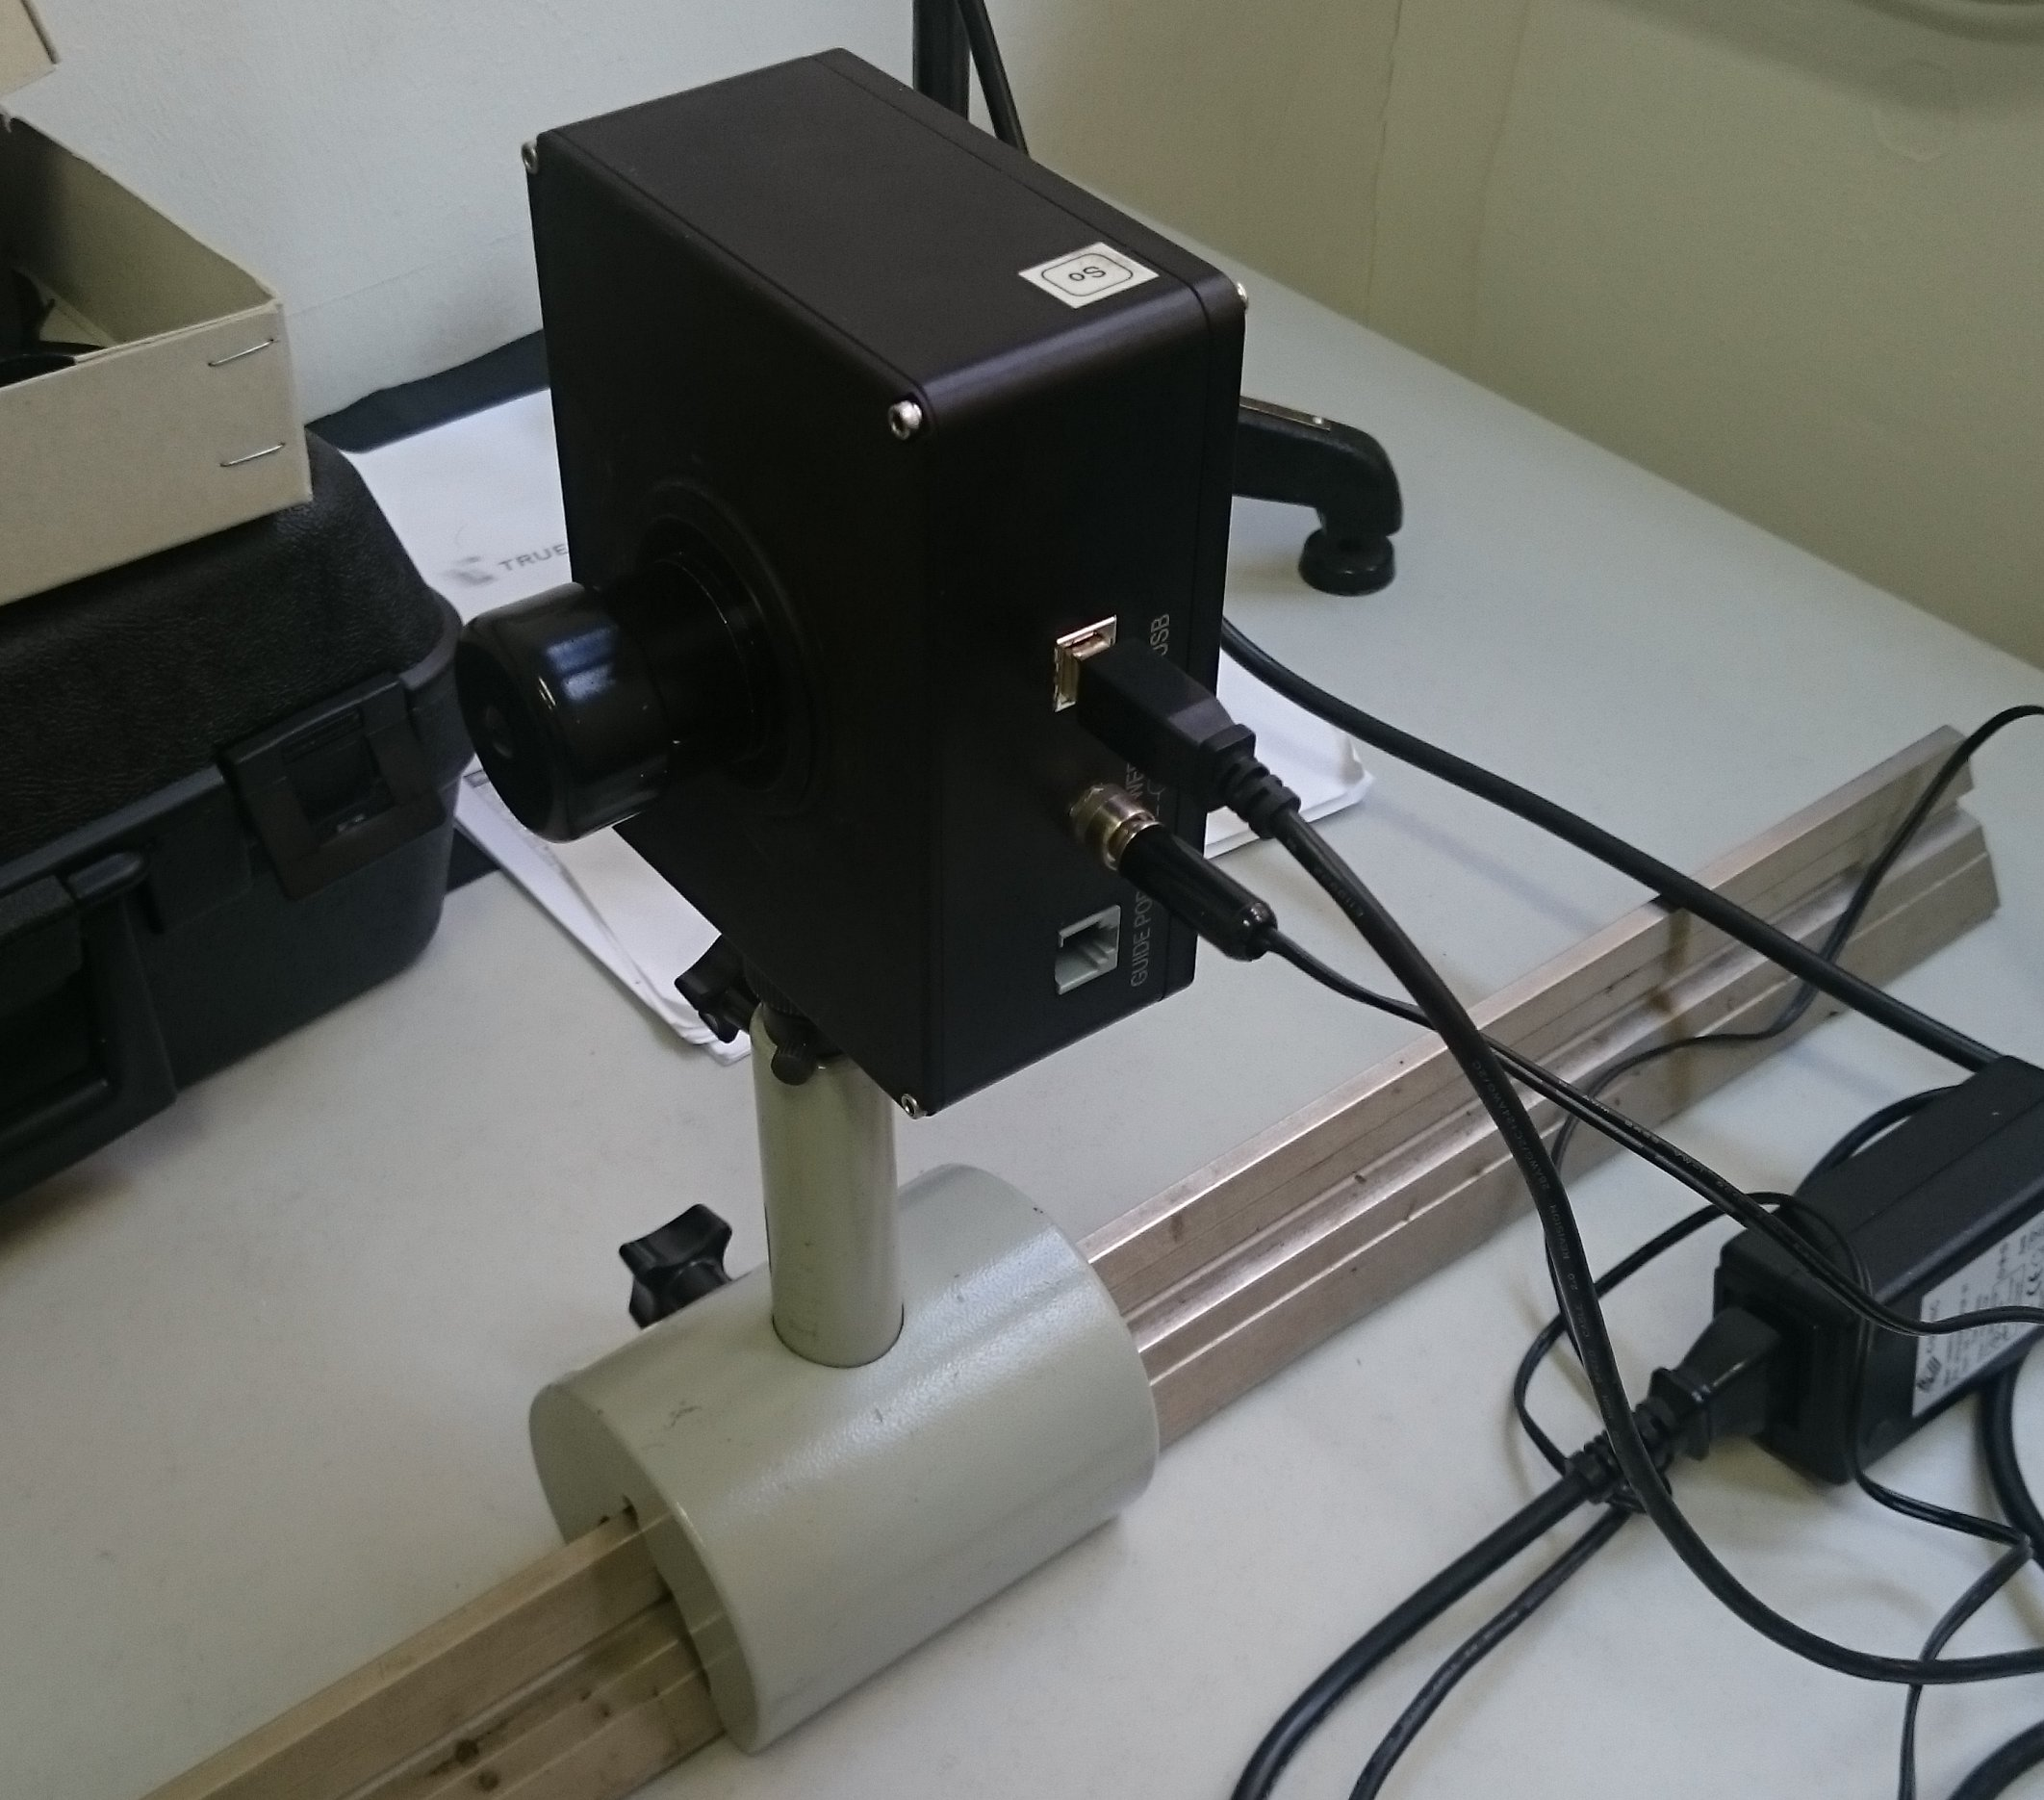
\includegraphics[scale=0.085]{messwerte/ccd-sensor-1.jpg}
			\caption{CCD-Kamera mit geschlossener Blende und Abdeckung bei Aufnahme der Dunkelstrombilder}
			\label{ccd_solo}
		\end{figure}
	% subsection dunkelstromaufnahme (end)


	\subsection{Überprüfung der Linearität} % (fold)
	\label{sub:_berpr_fung_der_linearit_t}
	
		Um den linearen Zusammenhang zwischen eingestrahlter Energie und gemessenen CCD-Signal zu zeigen, wurden Bilder bei stets gleicher Beleuchtung aber von Bild zu Bild steigender Belichtungszeit aufgenommen.
		Die Beleuchtung erfolgte wie in Abbildung \ref{mikrolampe} zu sehen über eine Mikroskoplampe und durch eine Lochblende vor der Kamera um Überbelichtung zu vermeiden.

		\begin{figure}
			\center
			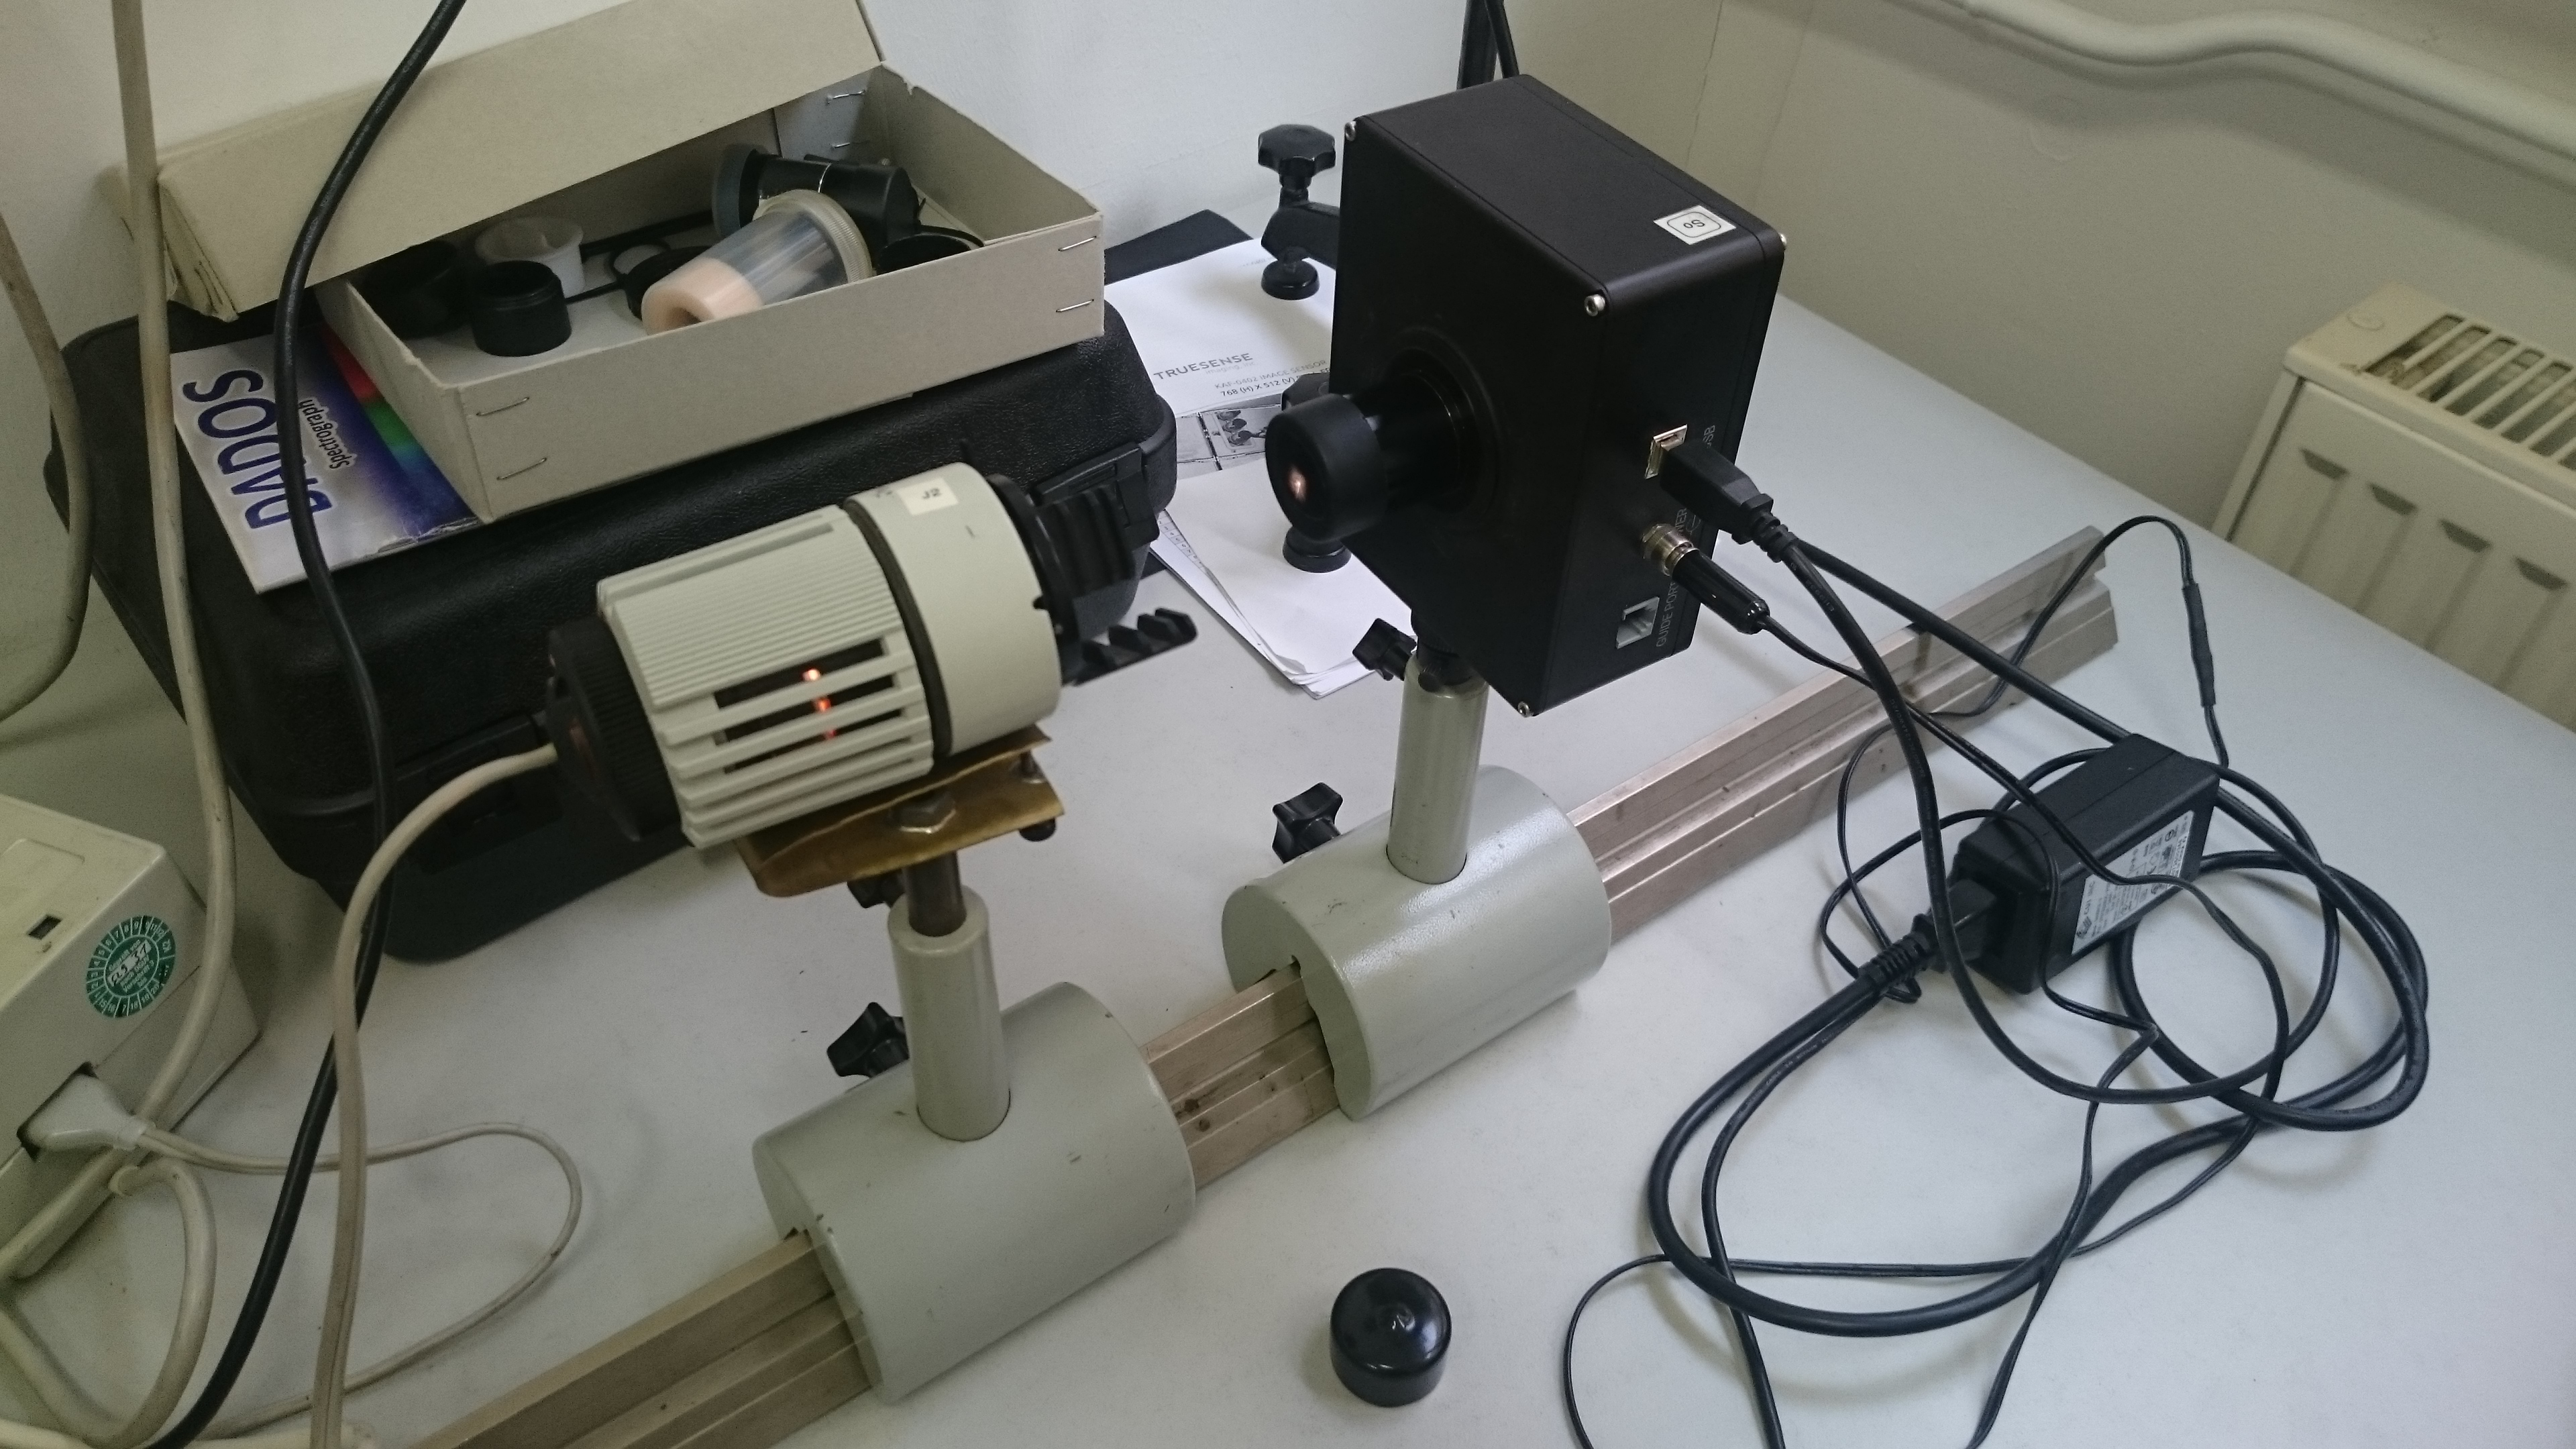
\includegraphics[scale=0.085]{messwerte/Handybilder/DSC_0671.JPG}
			\caption{CCD-Kamera mit beleuchteter Lochblende vor Mikroskoplampe zur Messung der Linearität}
			\label{mikrolampe}
		\end{figure}

	% subsection _berpr_fung_der_linearit_t (end)


	\subsection{Kalibrierung des Spektrometers} % (fold)
	\label{sub:kalibrierung_des_spektrometers}

		Um einen Zusammenhang zwischen beleuchteten CCD-Pixel und entsprechender Wellenlänge herzustellen, wurde vor jeder Aufnahme eines Sonnenspektrums zuerst ein Vergleichsspektrum einer bekannten Quelle aufgenommen.
		Die hierbei verwendeten Quellen waren eine Quecksilber-Cadmium-Entladungslampe sowie eine Neon-Glimmlampe.
		Ihre Spektren befinden sich unter \ref{sec:beispiele_des_sonnenspektrums} im Anhang am Ende des Protokolls.
		Ein Foto der Hg-Cd-Lampe, sowie der abbildenden Optik samt Gitter und angeschlossener CCD-Kamera ist in Abbildung \ref{hg_cd_lampe} zu sehen:

		\begin{figure}
			\center
			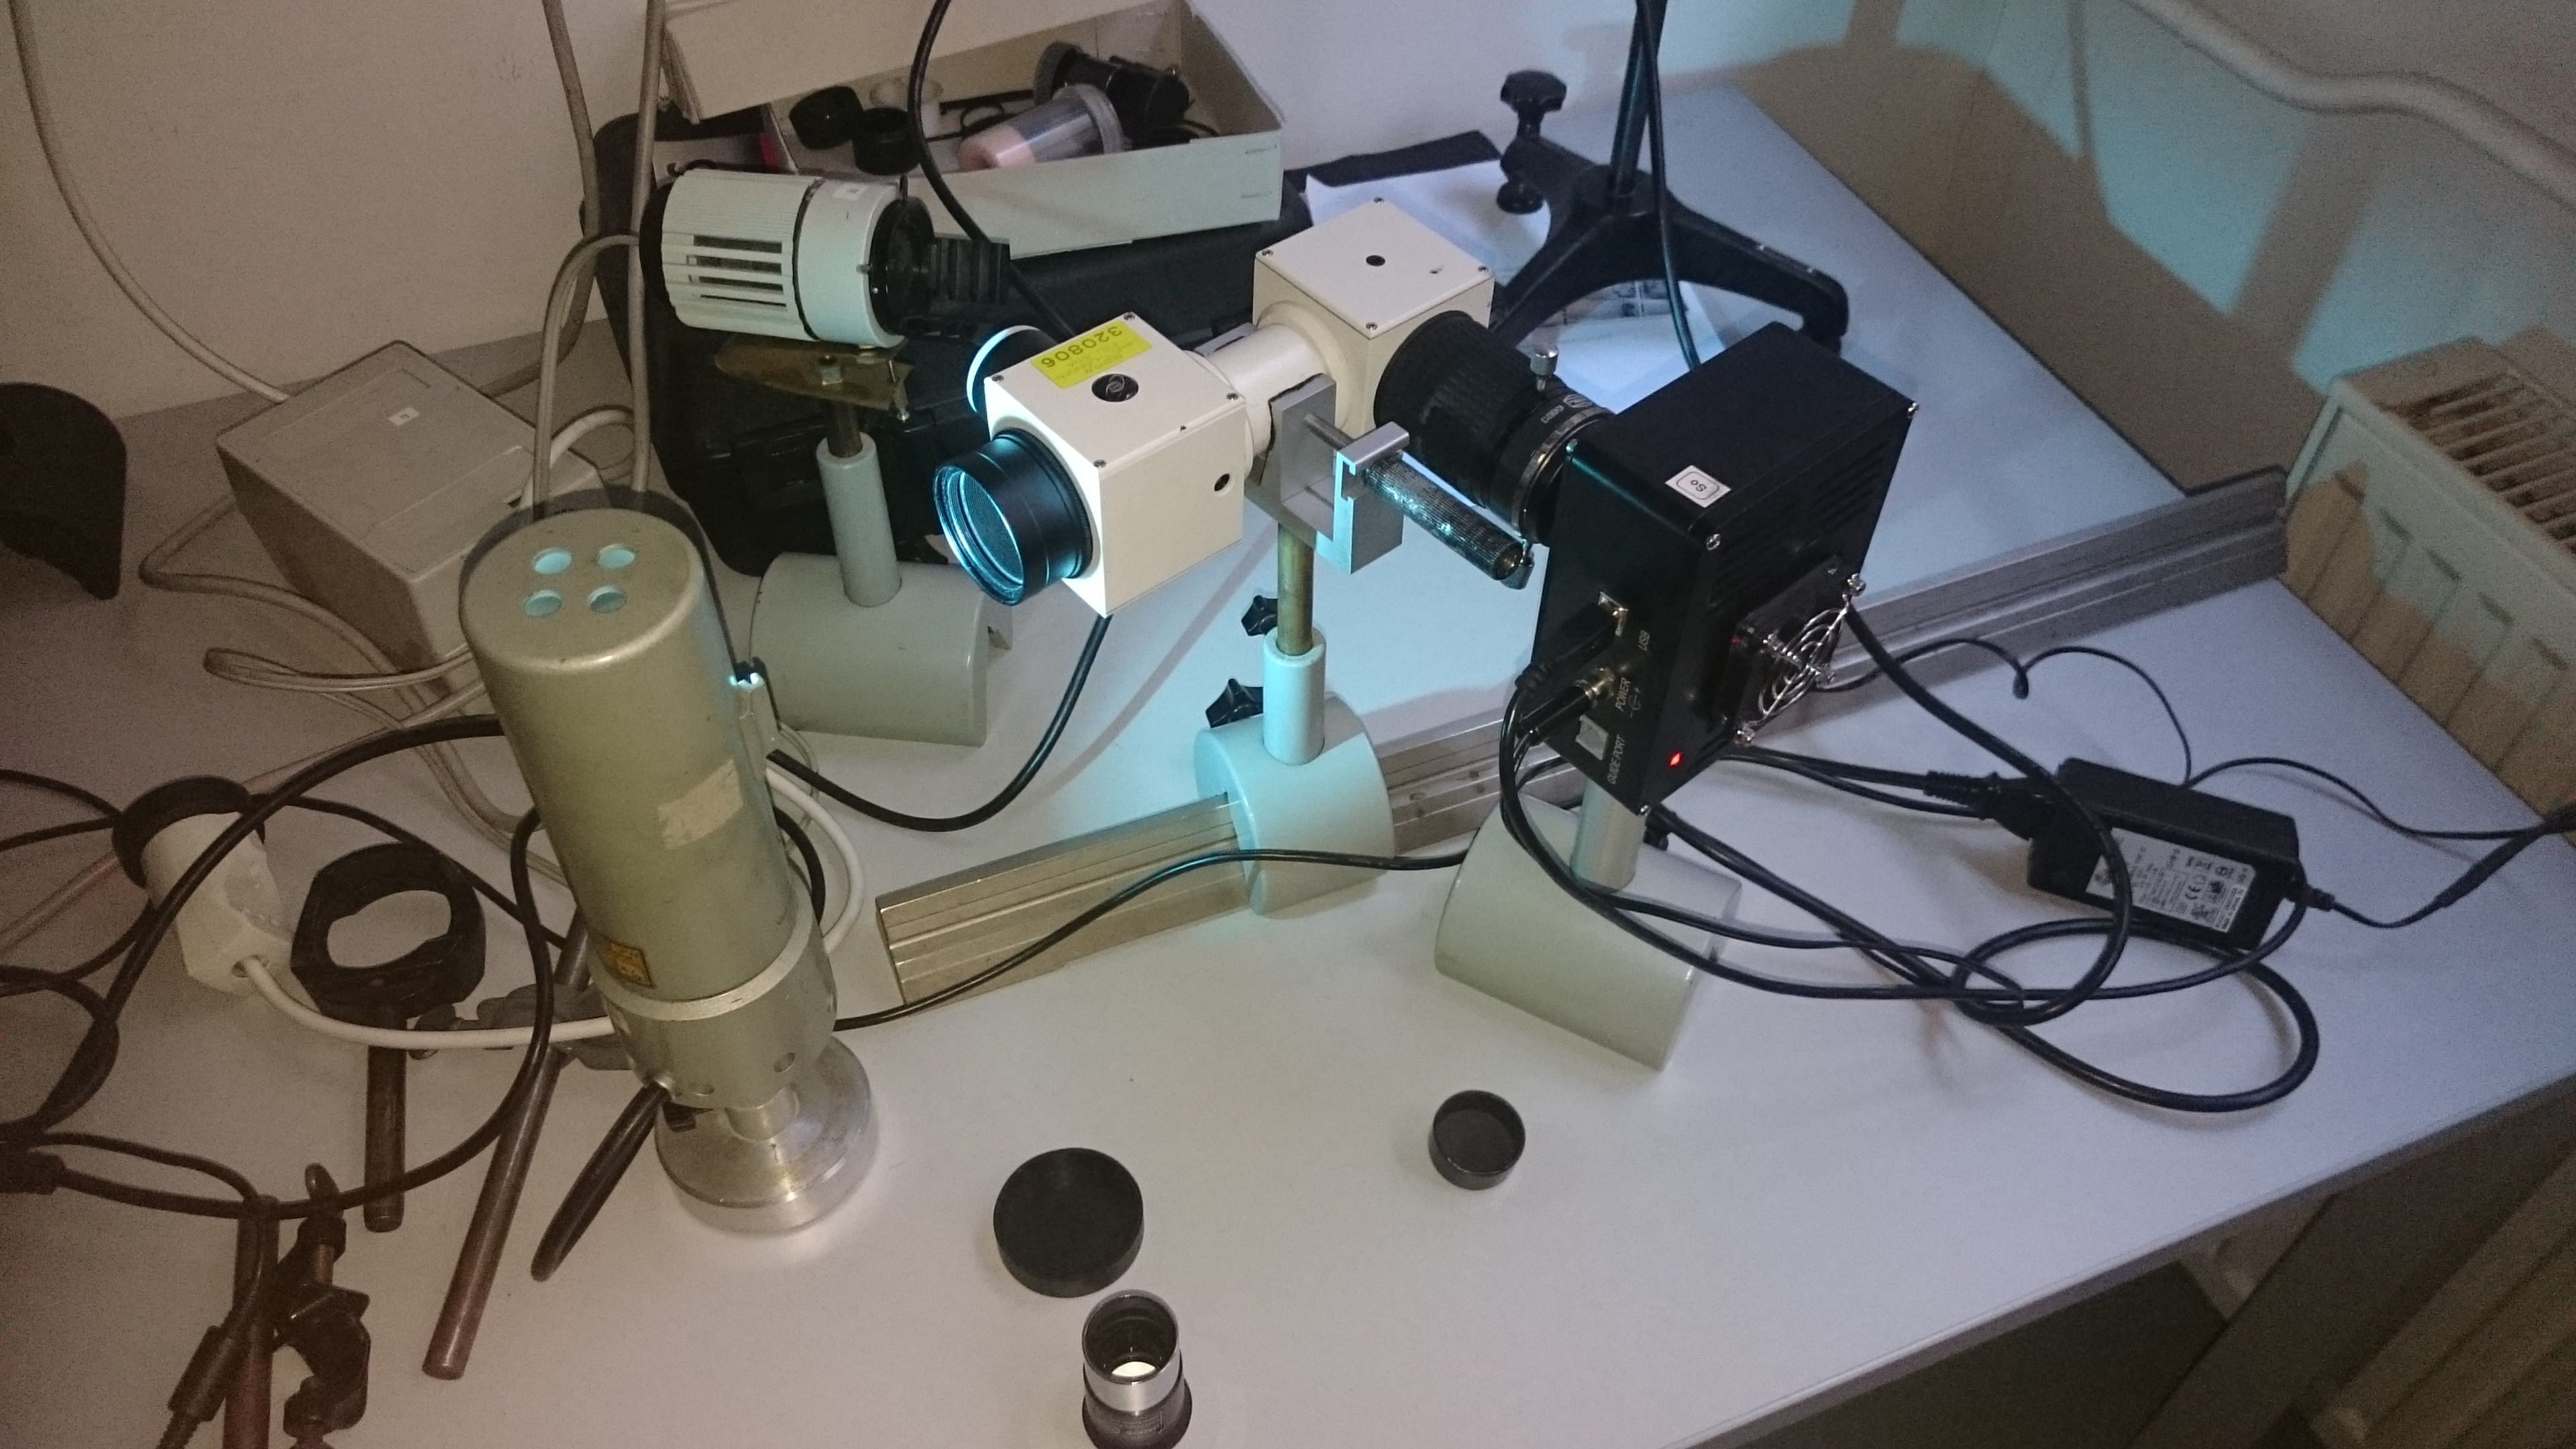
\includegraphics[scale=0.085]{messwerte/Handybilder/DSC_0675.JPG}
			\caption{von links nach rechts: Quecksilber-Cadmium-Lampe, abbildende Optik mit Gitter und CCD-Kamera bei Aufnahme eines Vergleichsspektrums}
			\label{hg_cd_lampe}
		\end{figure}


		\subsection{Aufnahme des Sonnenspektrums} % (fold)
		\label{sub:aufnahme_des_sonnenspektrums}

			Die Aufnahme des Sonnenspektrums erfolgte analog zur Aufnahm der Vergleichsspektren.
			Das indirekte, gestreute Sonnenlicht wurde dabei aus dem Himmel über einen Umlenkspiegel auf das Gitter geleitet.
			Der prinzipielle Aufbau ist in Abbildung \ref{spiegel_und_sonne} dargestellt.

			\begin{figure}
				\center
				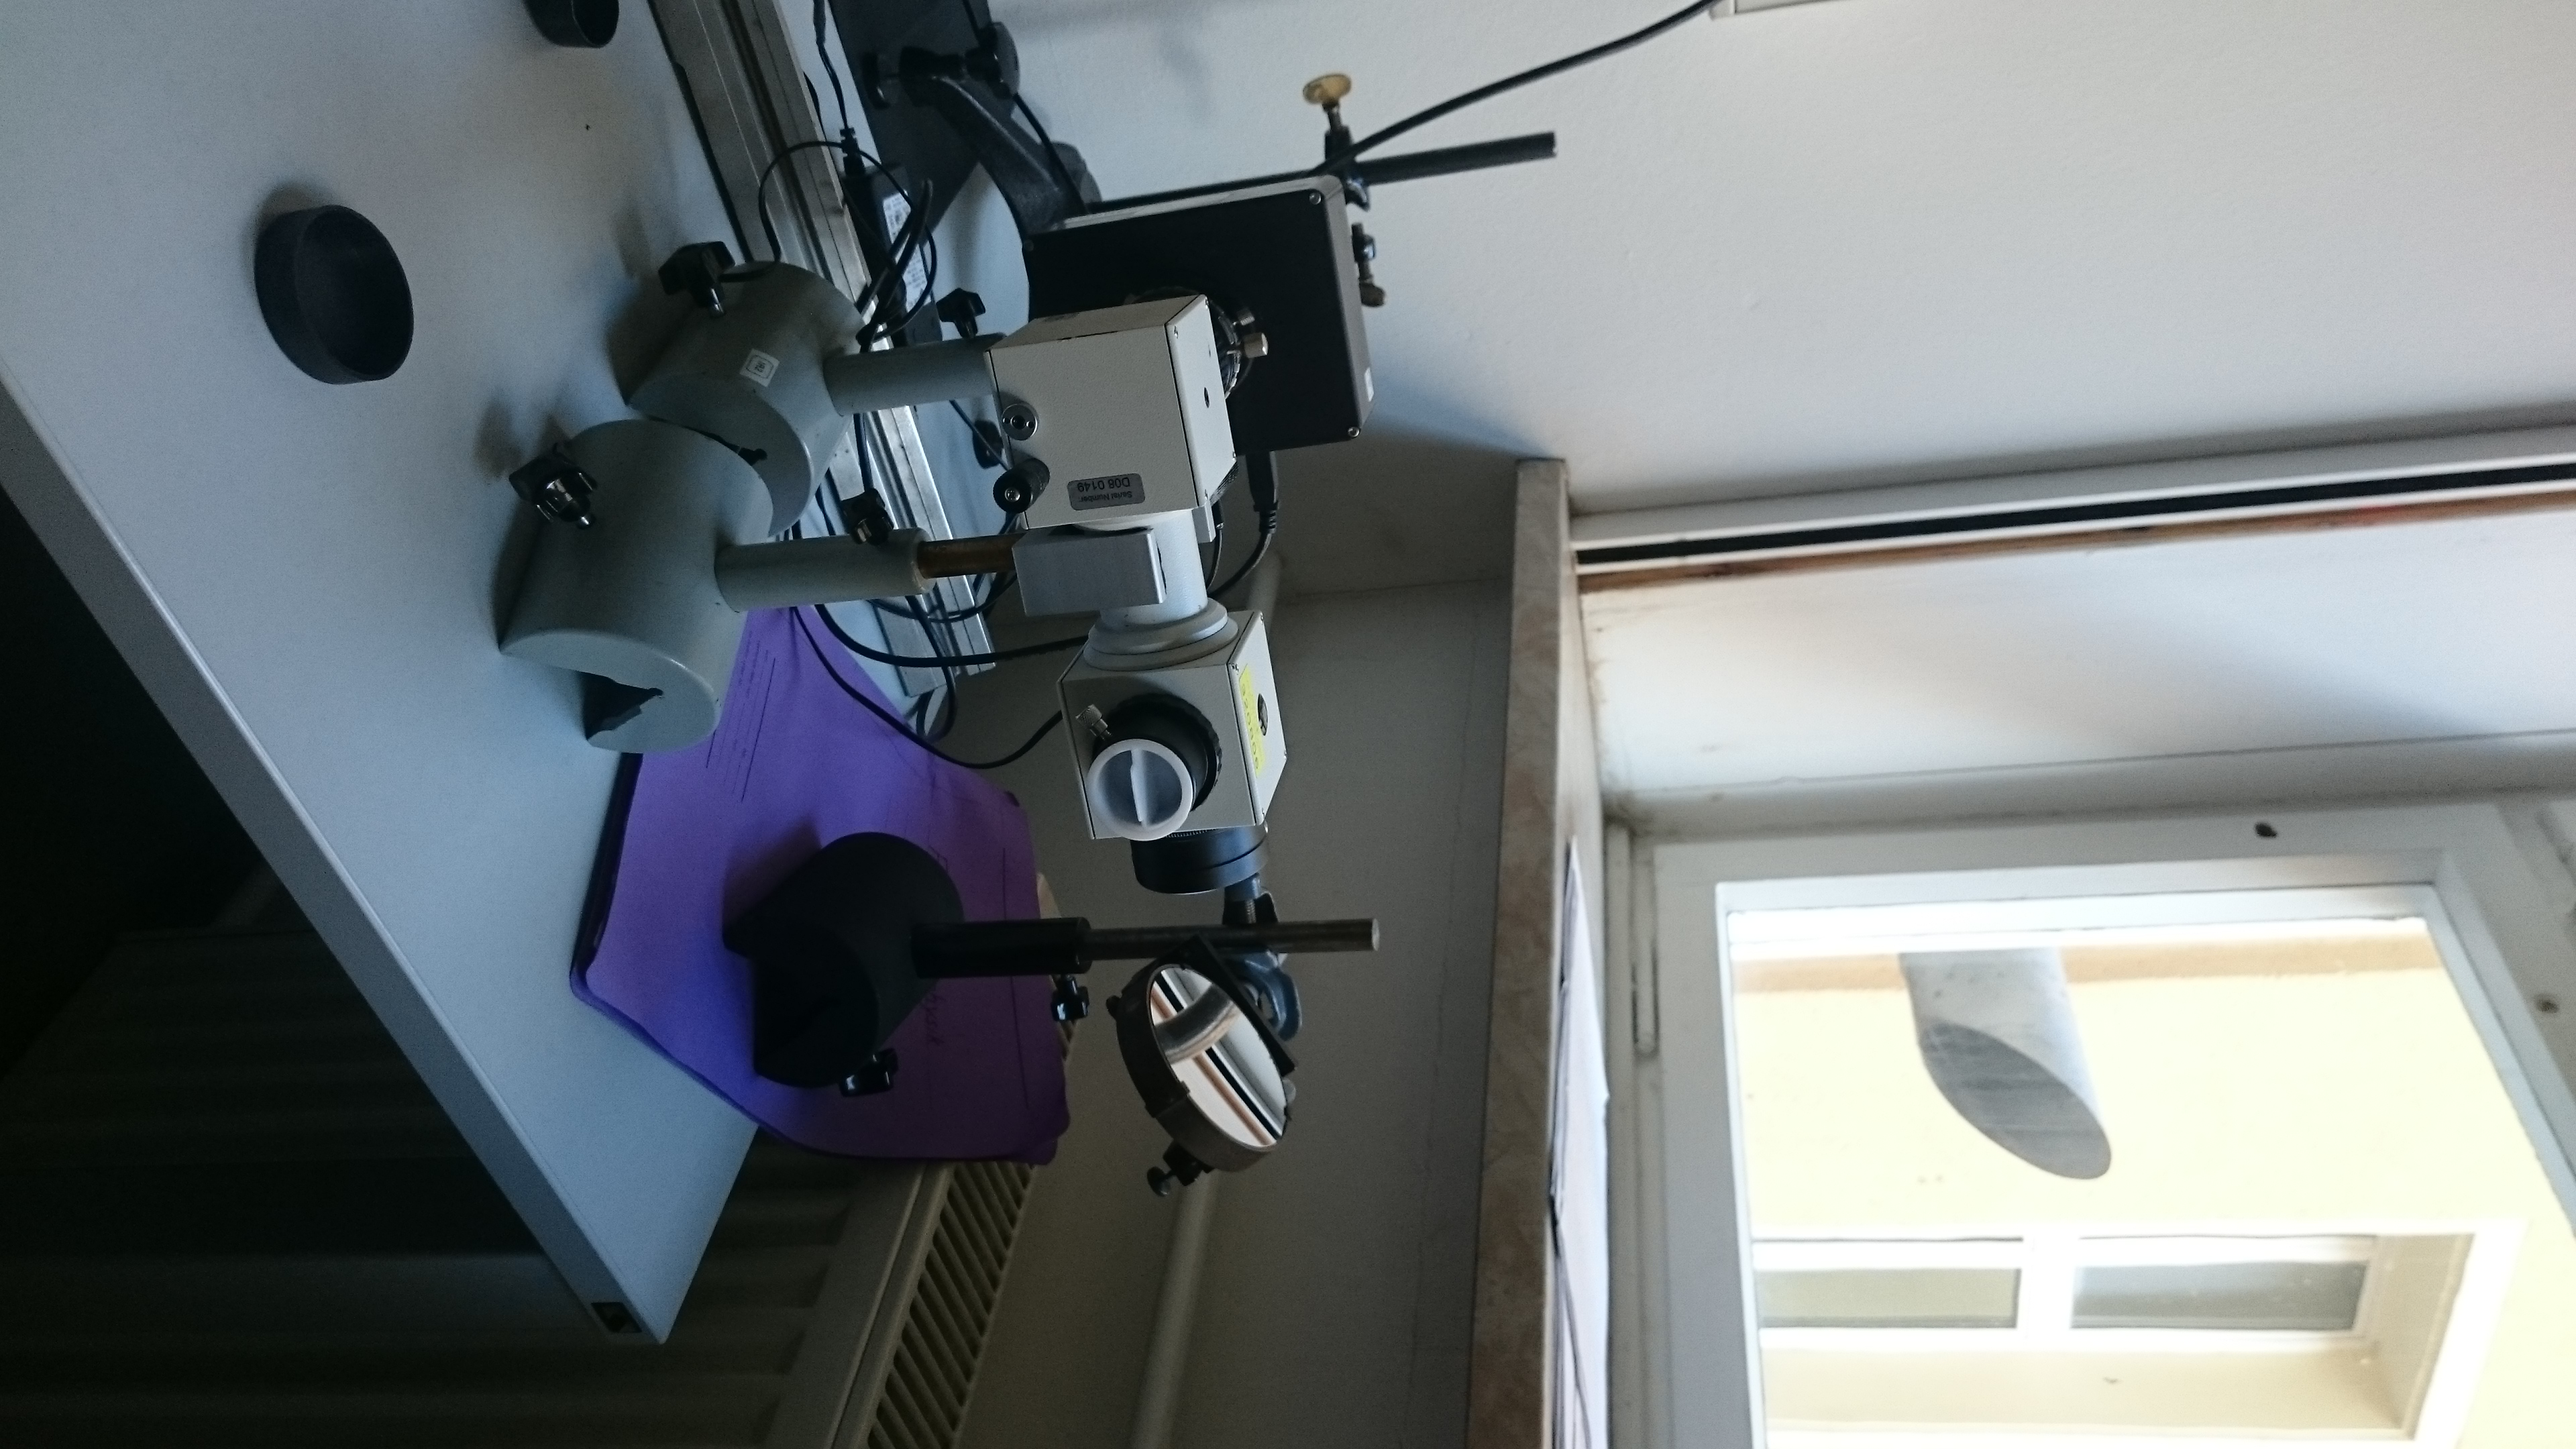
\includegraphics[scale=0.085]{messwerte/Handybilder/DSC_0694.JPG}
				\caption{Das durch das Fenster hereinstrahlende, gestreute Sonnenlicht wird über den Spiegel in die Optik und auf das Gitter geworfen, ehe das Spektrum mit der CCD-Kamera erfasst wird}
				\label{spiegel_und_sonne}
			\end{figure}

			Direkt im Anschluss an jede Spektrumsaufnahme, wurde der Spiegel durch eine der beiden Vergleichsquellen ersetzt und ein Bild zur Kalibrierung, sowie ein Biasbild aufgenommen.
			Durch Abzug des Biaslevels und Aufnahme bei $0\unit{$^\circ$C}$ konnten die systematischen Fehler gering gehalten werden.

		% subsection aufnahme_des_sonnenspektrums (end)

	% subsection kalibrierung_des_spektrometers (end)



% section aufbau_und_durchf_hrung (end)